While commuting zones are used by researchers as a convenient measure of local labor markets, they have a number of shortcomings for empirical research that are not regularly discussed in the literature. In this section, we evaluate the sensitivity of commuting zone definitions, focusing on two aspects of the TS1996 methodology. First, we show that if there is uncertainty in the input data, the resulting commuting zone definitions can vary substantially. Second, the resulting clusters are sensitive to the decision of when to stop merging clusters, which implies that small changes in the chosen cutoff height can affect the number and size of the clusters. Overall, this uncertainty and subjectivity in the commuting zone definitions contributes to conventional standard errors understating the true level of uncertainty in the estimates, which we show when we return to this issue with our empirical replication in the next section.

\subsection{Sensitivity of Clustering Results to Underlying Error}

Given the reliance of TS1996 on the commuting flows data, we want to analyze the extent to which the outputs of the TS1996 methodology are sensitive to errors in this data. First, recall equation \ref{eqn:diss} for the entries of the dissimilarity matrix. If $f_{ij}$ is measured without error, then the distance between counties $i$ and $j$ is also measured without error. However, if the flows are measured with error, $\epsilon_{ij}$, then we actually have an estimate of $D_{ij}$, which is $\hat{D}_{ij}$, which can be expressed as below (assuming without loss of generality that $rlf_i < rlf_j$):


\begin{align*}
\hat{D}_{ij} &= 1 - \frac{f_{ij} + \epsilon_{ij} + f_{ji} + \epsilon_{ji}}{\hat{rlf}_i} \\
&= 1- \frac{f_{ij} + f_{ji}}{rlf_{ij} + \sum_j \epsilon_{ij}} +  \frac{\epsilon_{ij} + \epsilon_{ji}}{rlf_{ij} + \sum_j \epsilon_{ij}}
\end{align*}

We assume that $E[\epsilon_{ij}]=0$ and that $\epsilon_{ij} \perp \epsilon_{ik} \forall k$. However, even if $E[\epsilon_{ij}]=0$, that does not imply that $E[\hat{D}_{ij}] = D_{ij}$. Furthermore, we cannot rely on the limit properties of the error distribution, because we only have one realization of the commuting flow, which is calculated from survey responses. Additionally, we know that $\frac{\epsilon_{ij}}{f_{ij}}$ is larger for small flows. This will increase $D_{ij}$ for some small counties and decrease it for others. Because of the hierarchical nature of the clustering method, this error will affect the formation of all other clusters in the data.\footnote{Additionally, because heights are normalized in the procedure, it also affects where the effective cutoff is, even for counties unaffected by errors in flows.}

To demonstrate how this measurement error affects the outcome of the clustering procedure, we use the published margins of error (MOE) from the 2009-2013 ACS Journey to Work data to calculate the ratio $MOE_{ij}/f_{ij}$ for different sized flows.\footnote{These flow size bins are the following percentile bins: 0-50; 50-90; 90-95; 95-99; and 99+.} We project these ratios onto the flow bins from the 1990 Journey to Work data (which does not publish margins of error), to have an estimated MOE.\footnote{There are other possible projections of the margins of error from one dataset to another. The Census Long form is designed to be a one-in-six sample for one year, while the ACS 5-year summary is designed to 5 years with a one-in-fifty sample each year. The smaller sample size typically results in higher margins of error in the ACS for comparable statistics. The uncertainty implied be our implementation may be thought of as an upper bound.} Using these estimated MOEs, we then obtain different realizations of the commuting zones in the following way:

\begin{enumerate}
	\item For each origin-destination pair ($i,j$), we draw $\epsilon_{ij}$ from a normal distribution with mean 0 and standard deviation $MOE_{ij}/(2 \times 1.64)$, since the MOE is the 90\% confidence interval.
	\item Calculate the new flow value, $\hat{f_{ij}} = f_{ij} + \epsilon_{ij}$, with negative values set to zero.
	\item Re-calculate each dissimilarity matrix entry $\hat{D}_{ij}$. 
	\item Re-run the hierarchical clustering procedure, using the same cutoff as the replication.
	\item Store the new clusters, and calculate the following statistics: average number of counties in a cluster; number of clusters; and total number of counties in a different cluster than the one they were originally assigned.
\end{enumerate}

We iterate over this procedure 1000 times in order to obtain distributions for these statistics. These graphs are shown in Figure \ref{fig:sensitivity}, where the red vertical dashed lines are the values that would be obtained using only the published figures. The figures show that the average cluster size varies considerably from the result the published figures would yield. Additionally, the share of the population that is mismatched is on average about 5\% of the US population, a small but non-negligible number. Overall, the underlying measurement error in the data causes uncertainty in the cluster definitions, which is exacerbated by the sharp cutoff imposed in cluster analysis.

\begin{figure}
\caption{Sensitivity Analysis \label{fig:sensitivity}}
\begin{tabular}{ccc}
%\includegraphics[scale=.5]{../figures/numclusters_jtw1990.png}& 
%\includegraphics[scale=.5]{../figures/mean_clussize_jtw1990.png}&
%\includegraphics[scale=.5]{../figures/mismatchedcounties_jtw1990.png} \\ 
(a) Number of clusters & (b) Average Number of Counties & (c) Mismatched Counties \\
\end{tabular}
\end{figure}

\subsection{Choosing Cluster Height}

Another sensitive feature of the methodology used by TS1996 is choosing the cutoff value above which no clusters can form. \cite{TK1987} describe the algorithm for choosing a cutoff value as follows (see page 15): ``As a rule of thumb, a normalized average distance of 0.98 was considered sufficient distance between sets of counties to treat them as separate [Labor Market Areas].'' The article does not provide an analysis of the sensitivity to changing the cutoff marginally up or down. \cite{TS1996}, in an effort to minimize methodological differences between commuting zones for 1980 and 1990, use the same cutoff with no further evaluation for the 1990 data. In this subsection, we investigate how sensitive the resulting clusters are to the choice of the cutoff value.

\begin{figure}
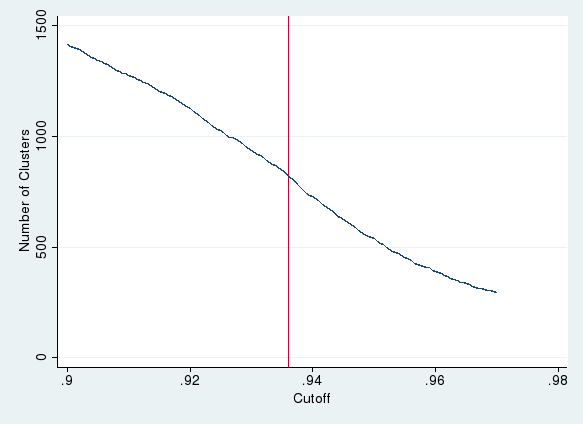
\includegraphics[scale=0.5]{./figures/numclus_cutoff.png}
\caption{Effect of Cluster Height on Number of Clusters \label{fig:cutoff_count}}
\emph{Note:} Authors' calculations using methodology outlined in Section \ref{sec:method}.
\end{figure}

Figure \ref{fig:cutoff_count} shows the number of clusters that form at various height cutoffs using the national 1990 JTW data, with the vertical line indicating the cutoff value we chose to replicate TS1990 (0.9418). The key takeaway from this figure is that it is theoretically ambiguous where a researcher should choose to stop merging clusters. Additionally, increasing or decreasing the cutoff has implications for the number of resulting clusters. Increasing it to 0.9428 decreases the number of clusters by 19, while using a cutoff of 0.9408 cause the number of clusters to increase by 17.

As we described above, the measurement error in commuting flows causes some uncertainty in terms of the true dissimilarity matrix, and hence the true cluster heights. Because of the presence of a strict cutoff, some clusters that would have formed if $D_{ij}$ were measured without error do not form, and vis-versa. More broadly, TS1996 provide no empirical guidance for choosing the optimal cutoff and cluster size other than referring to expert knowledge. While outside the scope of the current paper, future work may explore data-driven methods to determine whether there is an optimal number of clusters for certain uses.
